\section{1-DOF System}
We consider as transfer function from voltage to the mass speed:\\
\\
\[	
G(s)=
\frac{-5.618*10^{4}}{{s^3+21.45*s^{2}}+1699*s+3.149*10^{4}}
\]
\\


\begin{figure*}[h]
	\centering
	\begin{subfigure}{0.4\columnwidth}
		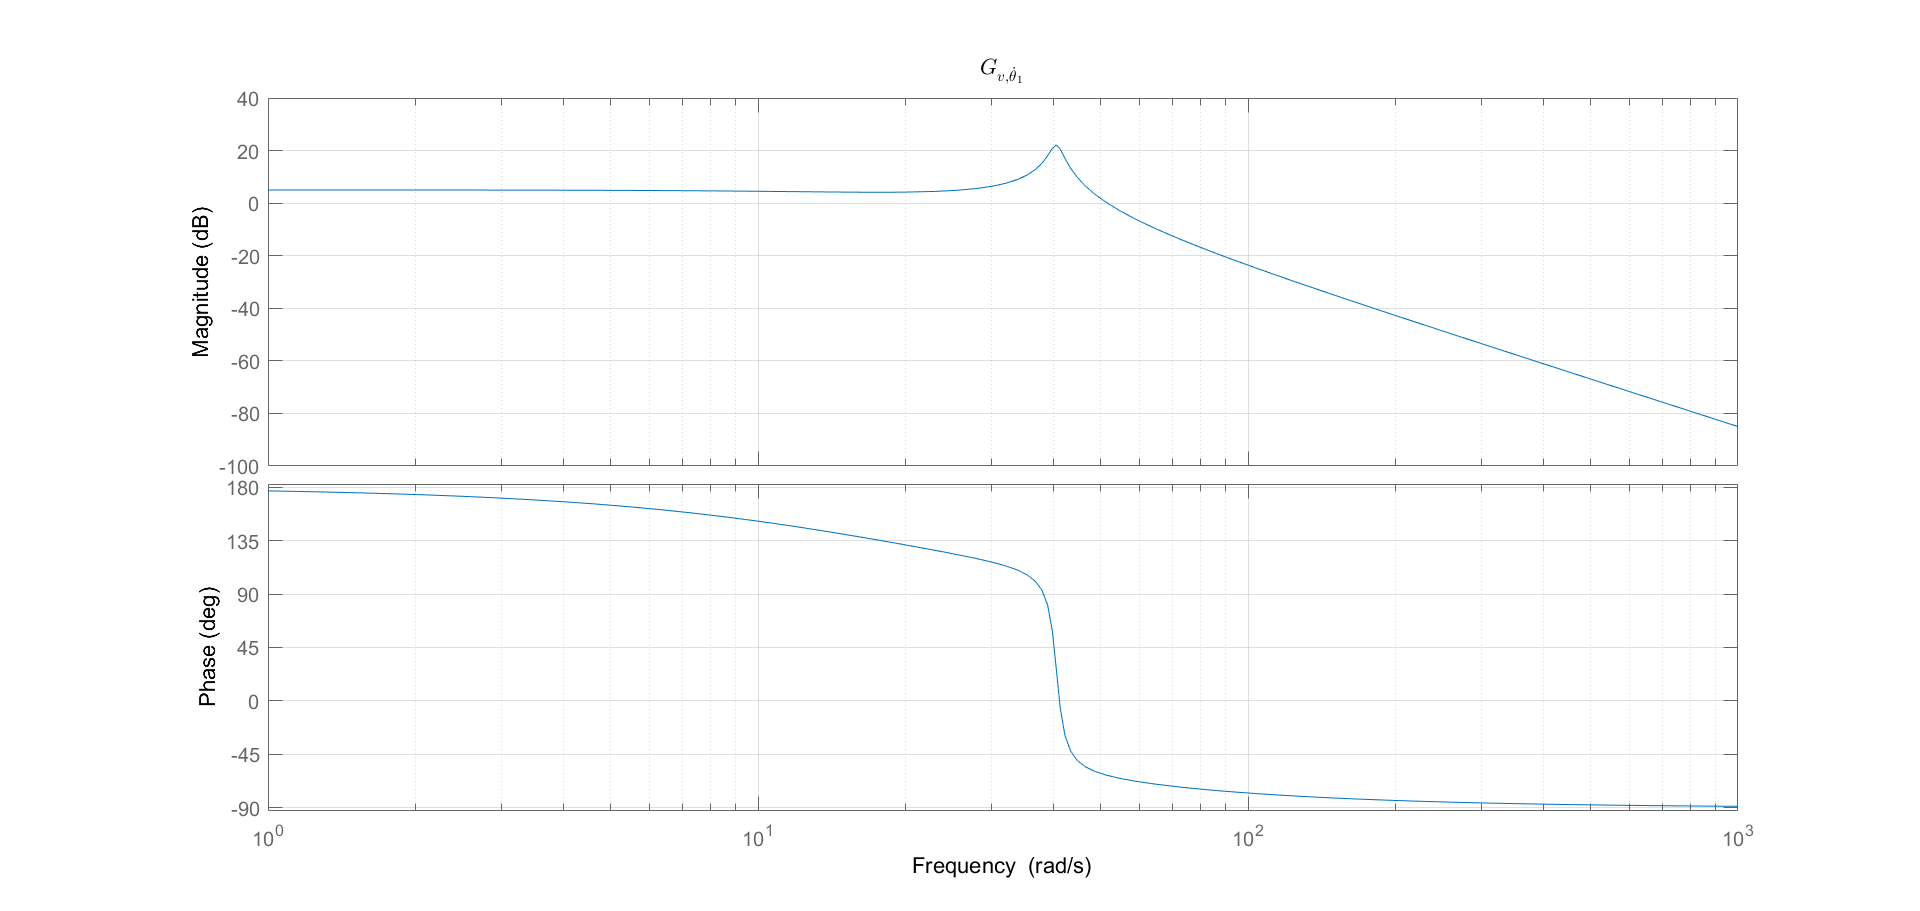
\includegraphics[width=\textwidth]{1Bode_G}
	\end{subfigure}
	\begin{subfigure}{0.4\columnwidth}
		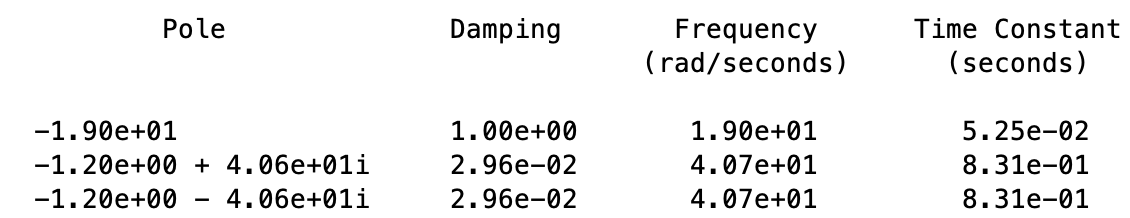
\includegraphics[width=\textwidth]{1Pole_G}
	\end{subfigure}
	\caption{G(s)}
	\label{fig:G(s)1dof}
\end{figure*}

As it is possible to notice in figure \ref{fig:G(s)1dof}, there is a couple of complex conjugated poles with low damping coefficient. We decide so to apply a notch filter, thanks to which we are able to delete these poles and substitute them with a couple of complex conjugated poles at the same frequency but with a damping coefficent equal to 0.72. We decide not to alter too much the behavior of the plant not to have a too aggressive control action, for this reason we do not impose real poles or high frequency poles.

\begin{figure*}[h]
	\centering
	\begin{subfigure}{0.35\columnwidth}
		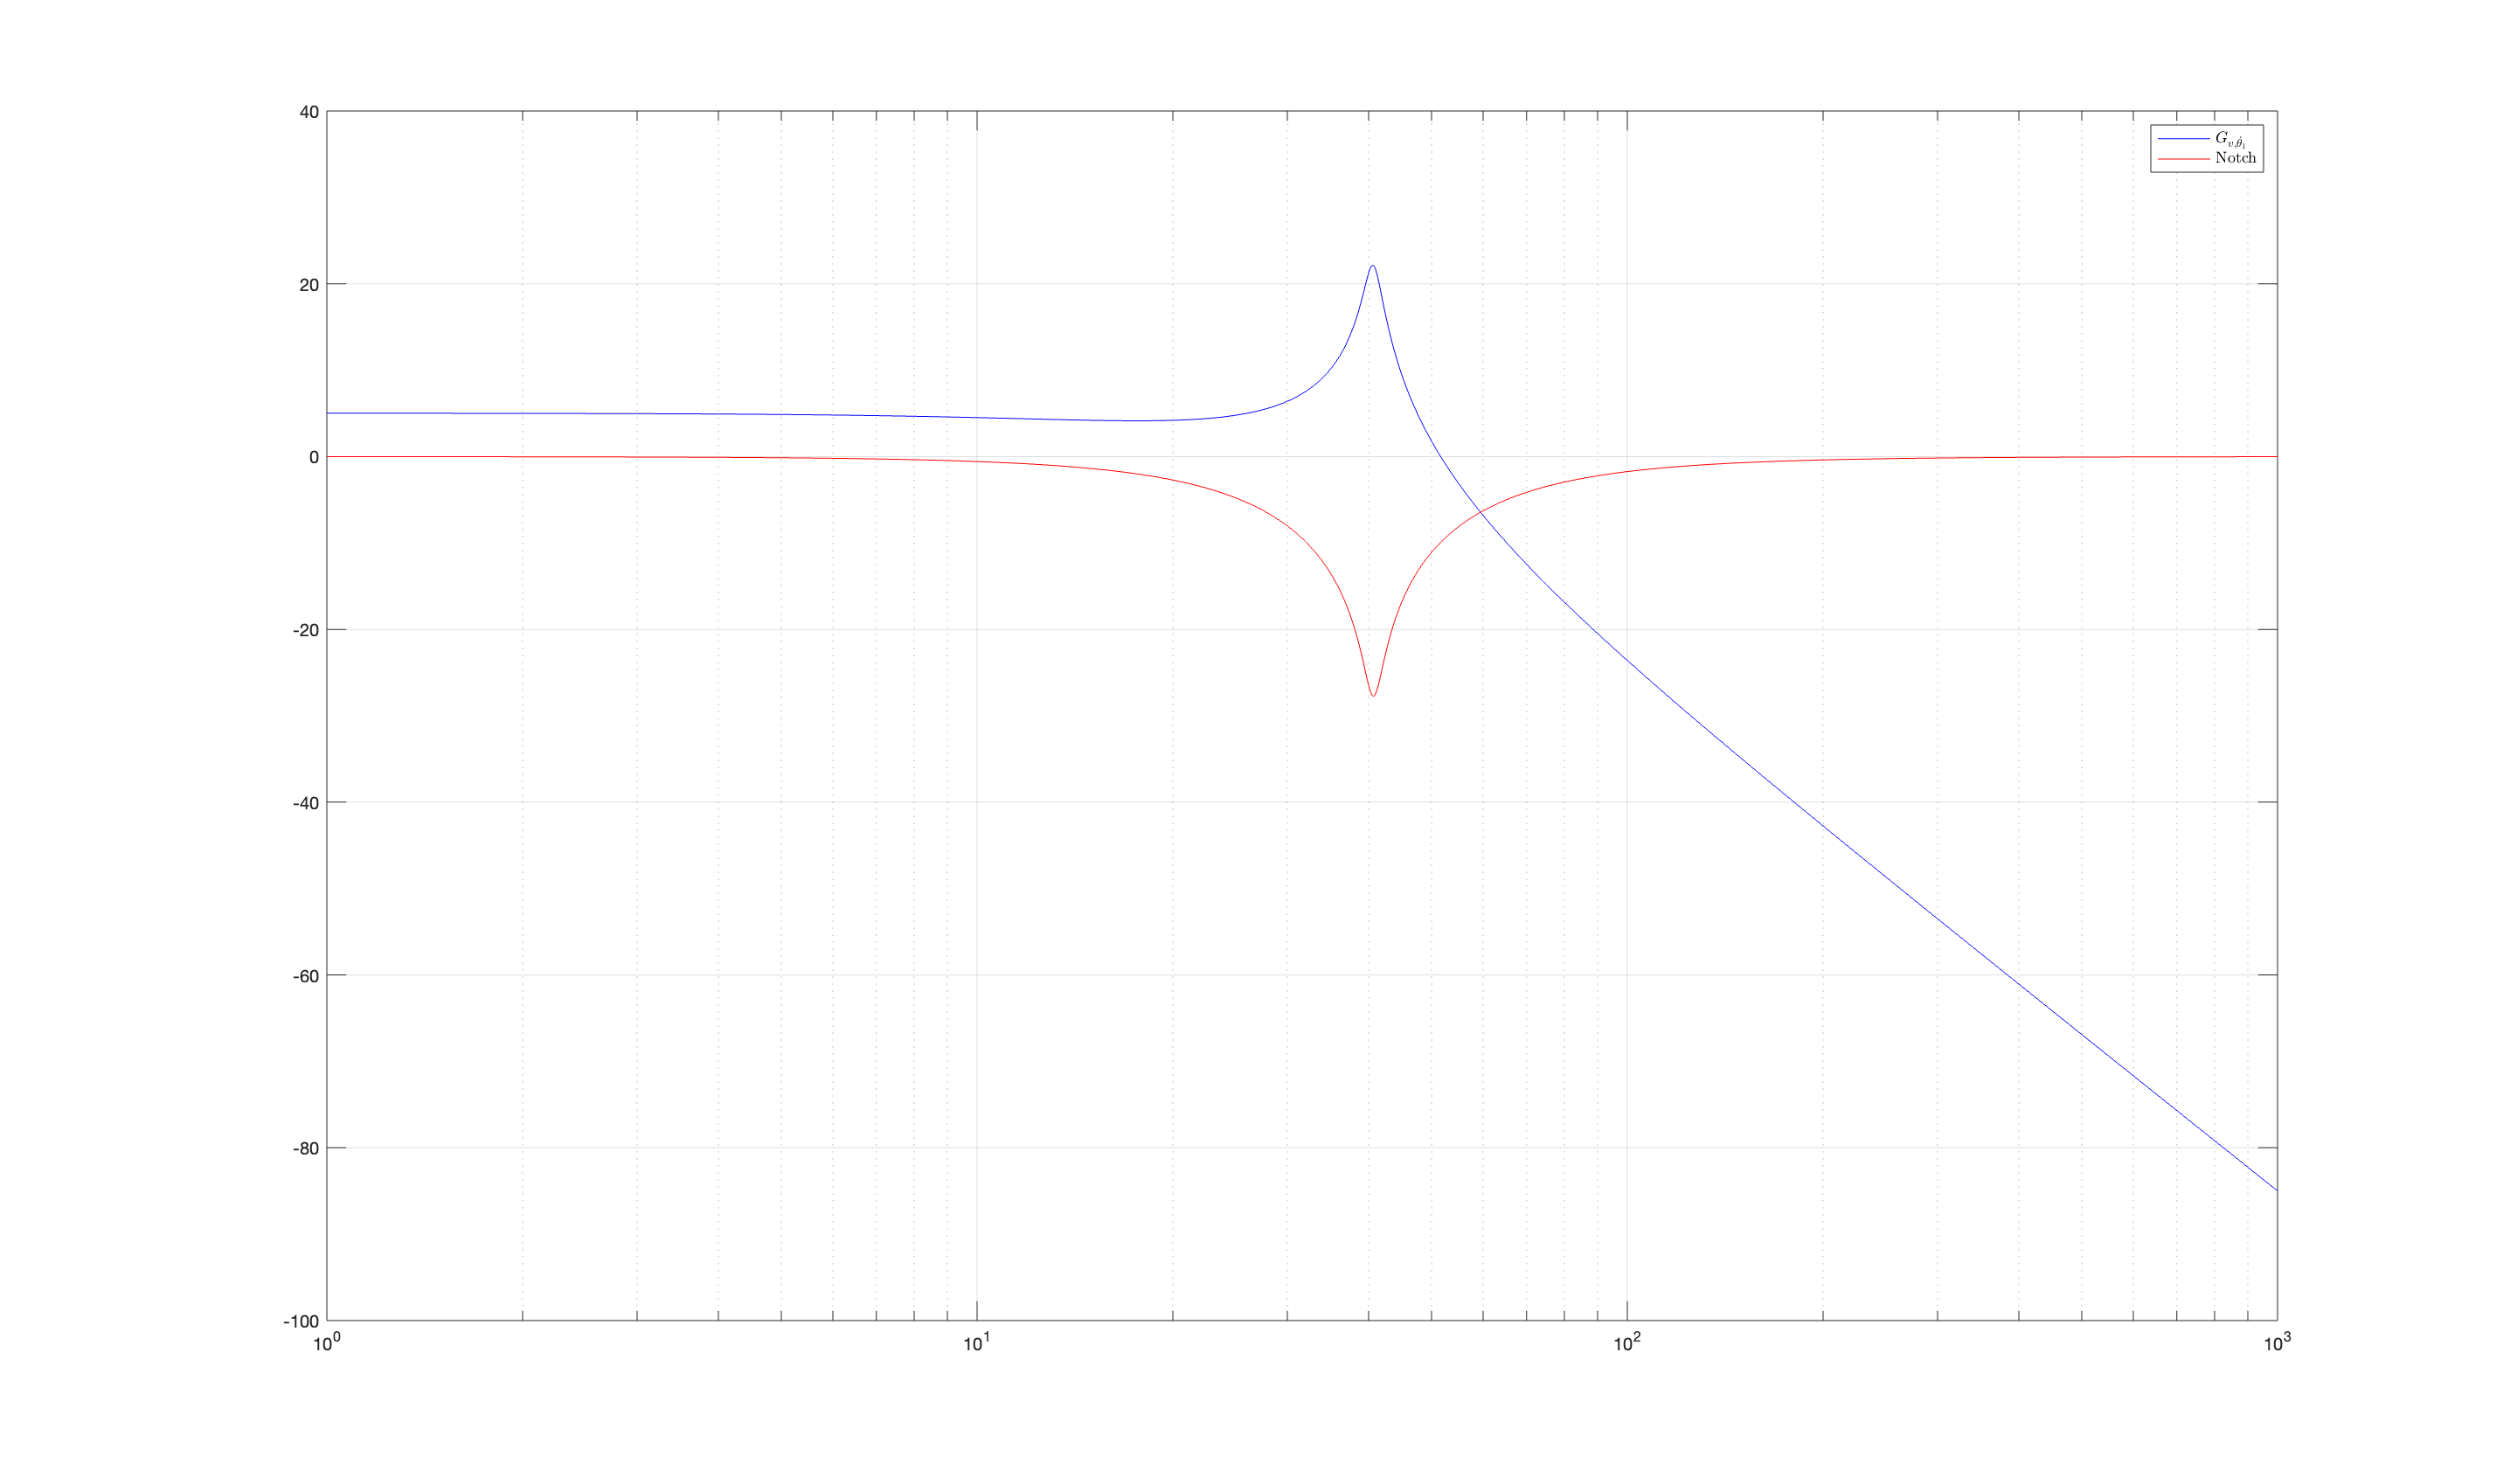
\includegraphics[width=\textwidth]{1Nf_G}
		\subcaption{Nf(s) and G(s)}
	\end{subfigure}
	\begin{subfigure}{0.35\columnwidth}
		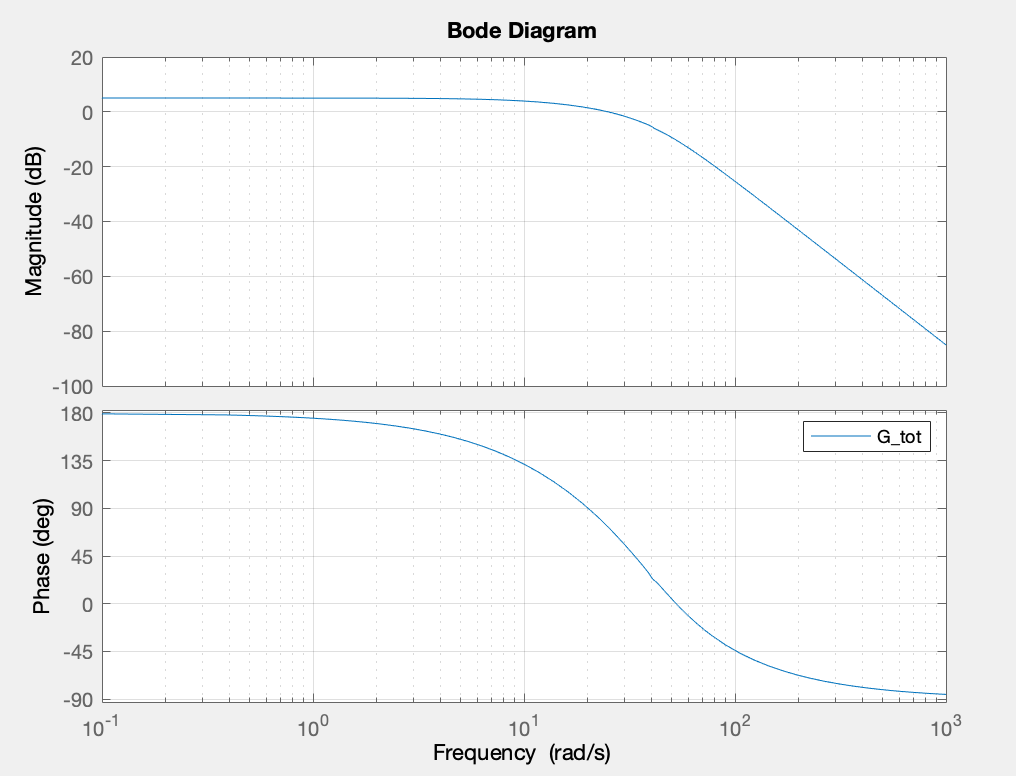
\includegraphics[width=\textwidth]{1_Gtot}
		\subcaption{$G_{tot}$(s)}
	\end{subfigure}
	\caption{Plant G(s) with Notch Filter Nf(s): $G_{tot}$(s)}
	\label{fig:Plant G(s)with Notch Filter1}
\end{figure*}


Applying the notch filter represented in figure \ref{fig:Plant G(s)with Notch Filter1}(a), we obtain the plant $G_{tot}$(s) of figure \ref{fig:Plant G(s)with Notch Filter1}(b) that is the one we are going to control.



\newpage
\subsection{Speed Control Loop}
We choose as regulator the PI controller enriched with an anti-windup structure, with which we cancel out the real frequency pole at 19 rad/s. \\
\\
\[
R(s)=-wc_v
\frac{\frac{s}{19}+1}{s}
\]
\\

We would like to have a cutting frequency at 10 rad/s,but we notice that, due to the presence of the notch-filter, the cutting frequency imposed by the PI-controller is postponed. For this reason, from now on we will use $wc_v$ only as the parameter set inside of the PI regulator and not to define the real bandwidth of the speed loop.
\\
\begin{figure*}[h]
	\centering
	\begin{subfigure}{0.45\columnwidth}
		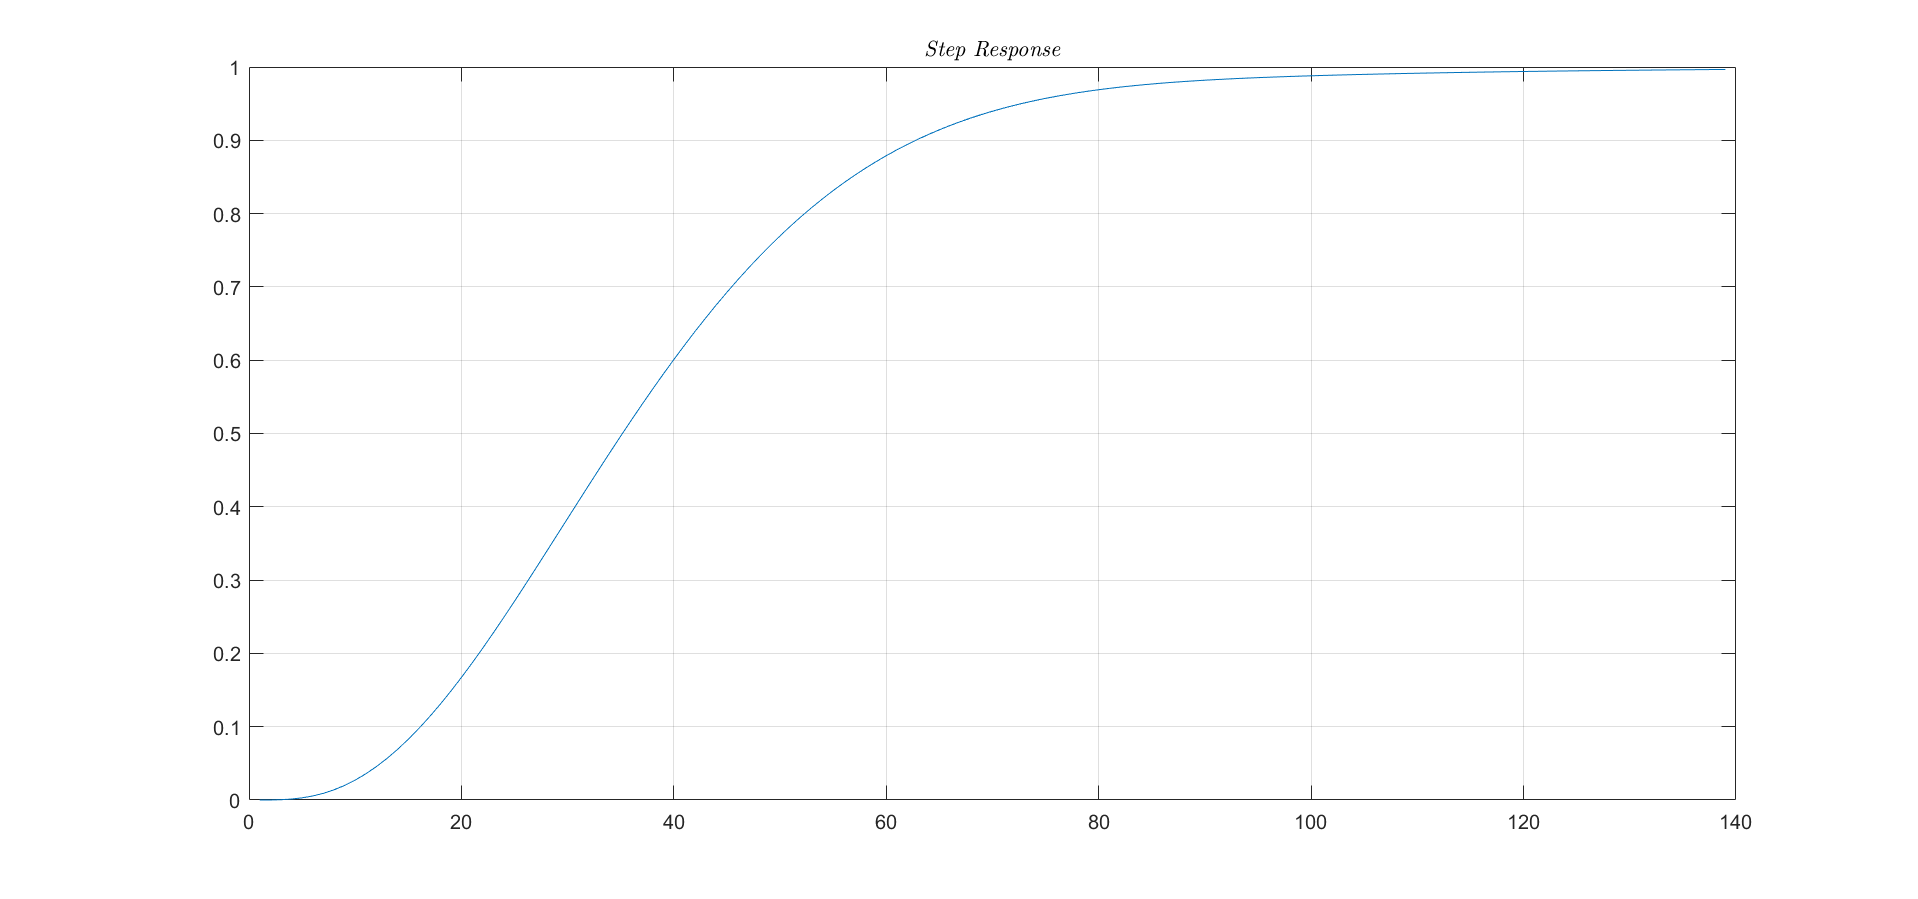
\includegraphics[width=\textwidth]{1step10}
	\end{subfigure}
	\begin{subfigure}{0.45\columnwidth}
		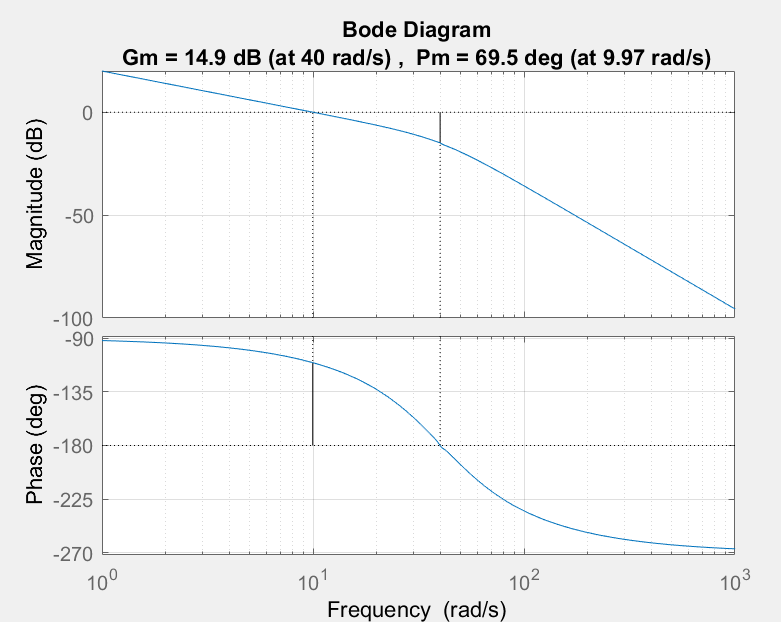
\includegraphics[width=\textwidth]{1bode10}
	\end{subfigure}
	\caption{Speed control loop with  $wc_{v} $=10 rad/s}
	\label{fig:Bode and Step PI 10}
\end{figure*}
\\
This open loop system would lead us to the step response of the figure \ref{fig:Bode and Step PI 10}. 
Even if this response could be considered acceptable, we have to remember that this is just a simulation. Having such a low phase margin could generate undesidered behavior in presence of disturbance of the real system. In order to have a more robust control system, it is so necessary to increase the phase margin by reducing the cutting frequency. 
\newline After many tests at the laboratory we choose for the best configuration which is obtained by setting $wc_{v} $=4.5. We consider this solution a good trade-off between the settling time and the robustness of the closed loop system.
We consider one of the worst case scenarios, that is the step from -17 rad/s to 17 rad/s, and then we apply a step of 10 rad/s. The first one lets us to asses the voltage saturation while the second one the transient after an ordinary step.
We plot them comparing the simulation and the data collected in the laboratory.


\begin{figure*}[h]
	\centering
	\begin{subfigure}{0.33\columnwidth}
		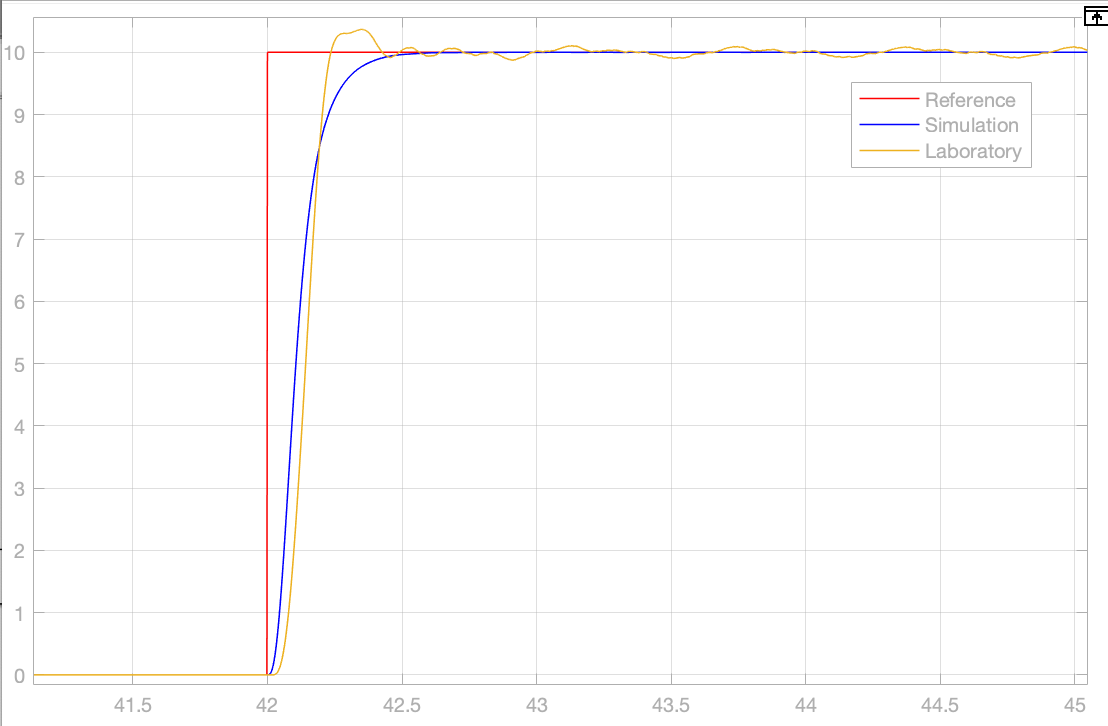
\includegraphics[width=\textwidth]{1_step10}
		\subcaption{Step 10 rad/s}
	\end{subfigure}
	\begin{subfigure}{0.33\columnwidth}
		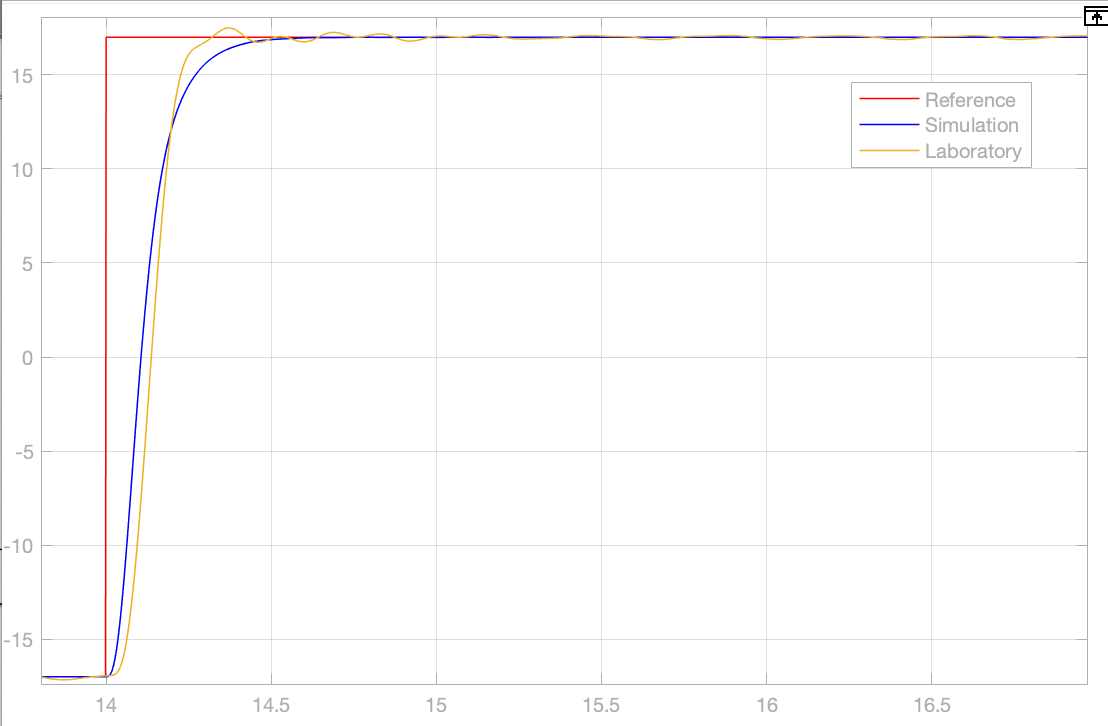
\includegraphics[width=\textwidth]{1_step17}
		\subcaption{Step 17 rad/s}
	\end{subfigure}
	\begin{subfigure}{0.32\columnwidth}
		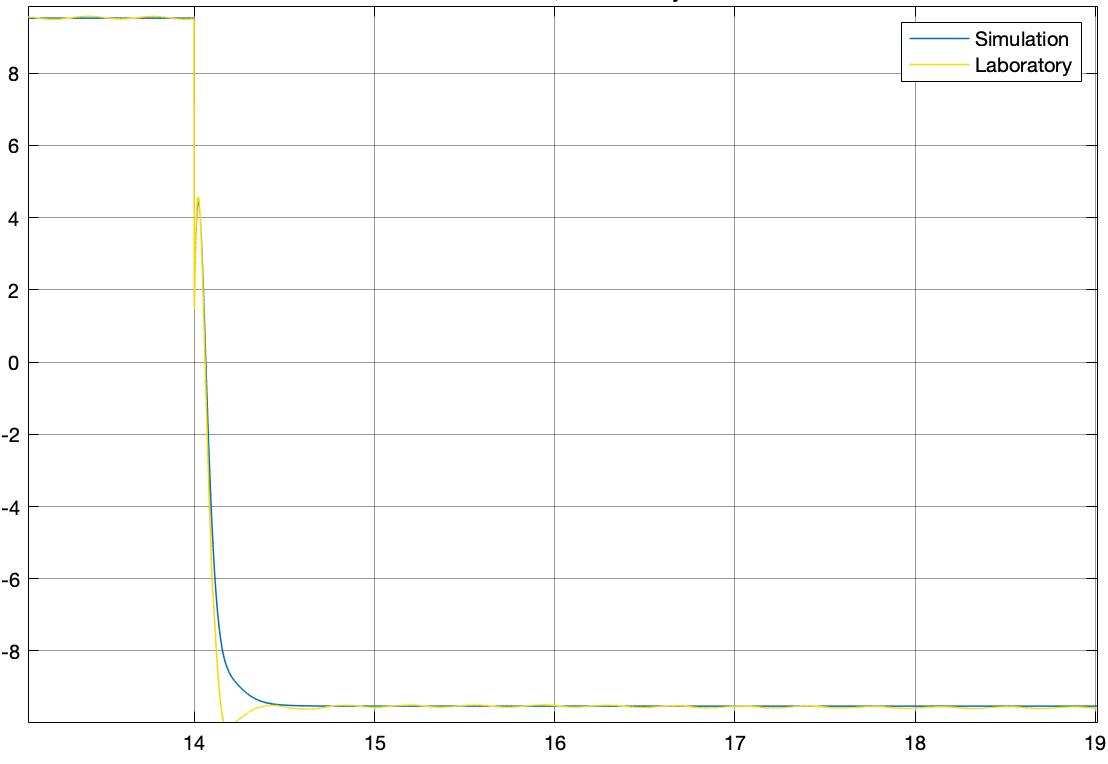
\includegraphics[width=\textwidth]{1_volt17}
		\subcaption{Voltage related to a step of 17 rad/s}
	\end{subfigure}
	\caption{Speed control loop with  $wc_{v} $=4.5 rad/s}
	\label{fig:PI with 4.5}
\end{figure*}

\newpage We plot now a sinesweep experiment to evaluate the bandwidth and a ramp reference with lowa slope to test the controllability range.

\begin{figure*}[h]
	\centering
	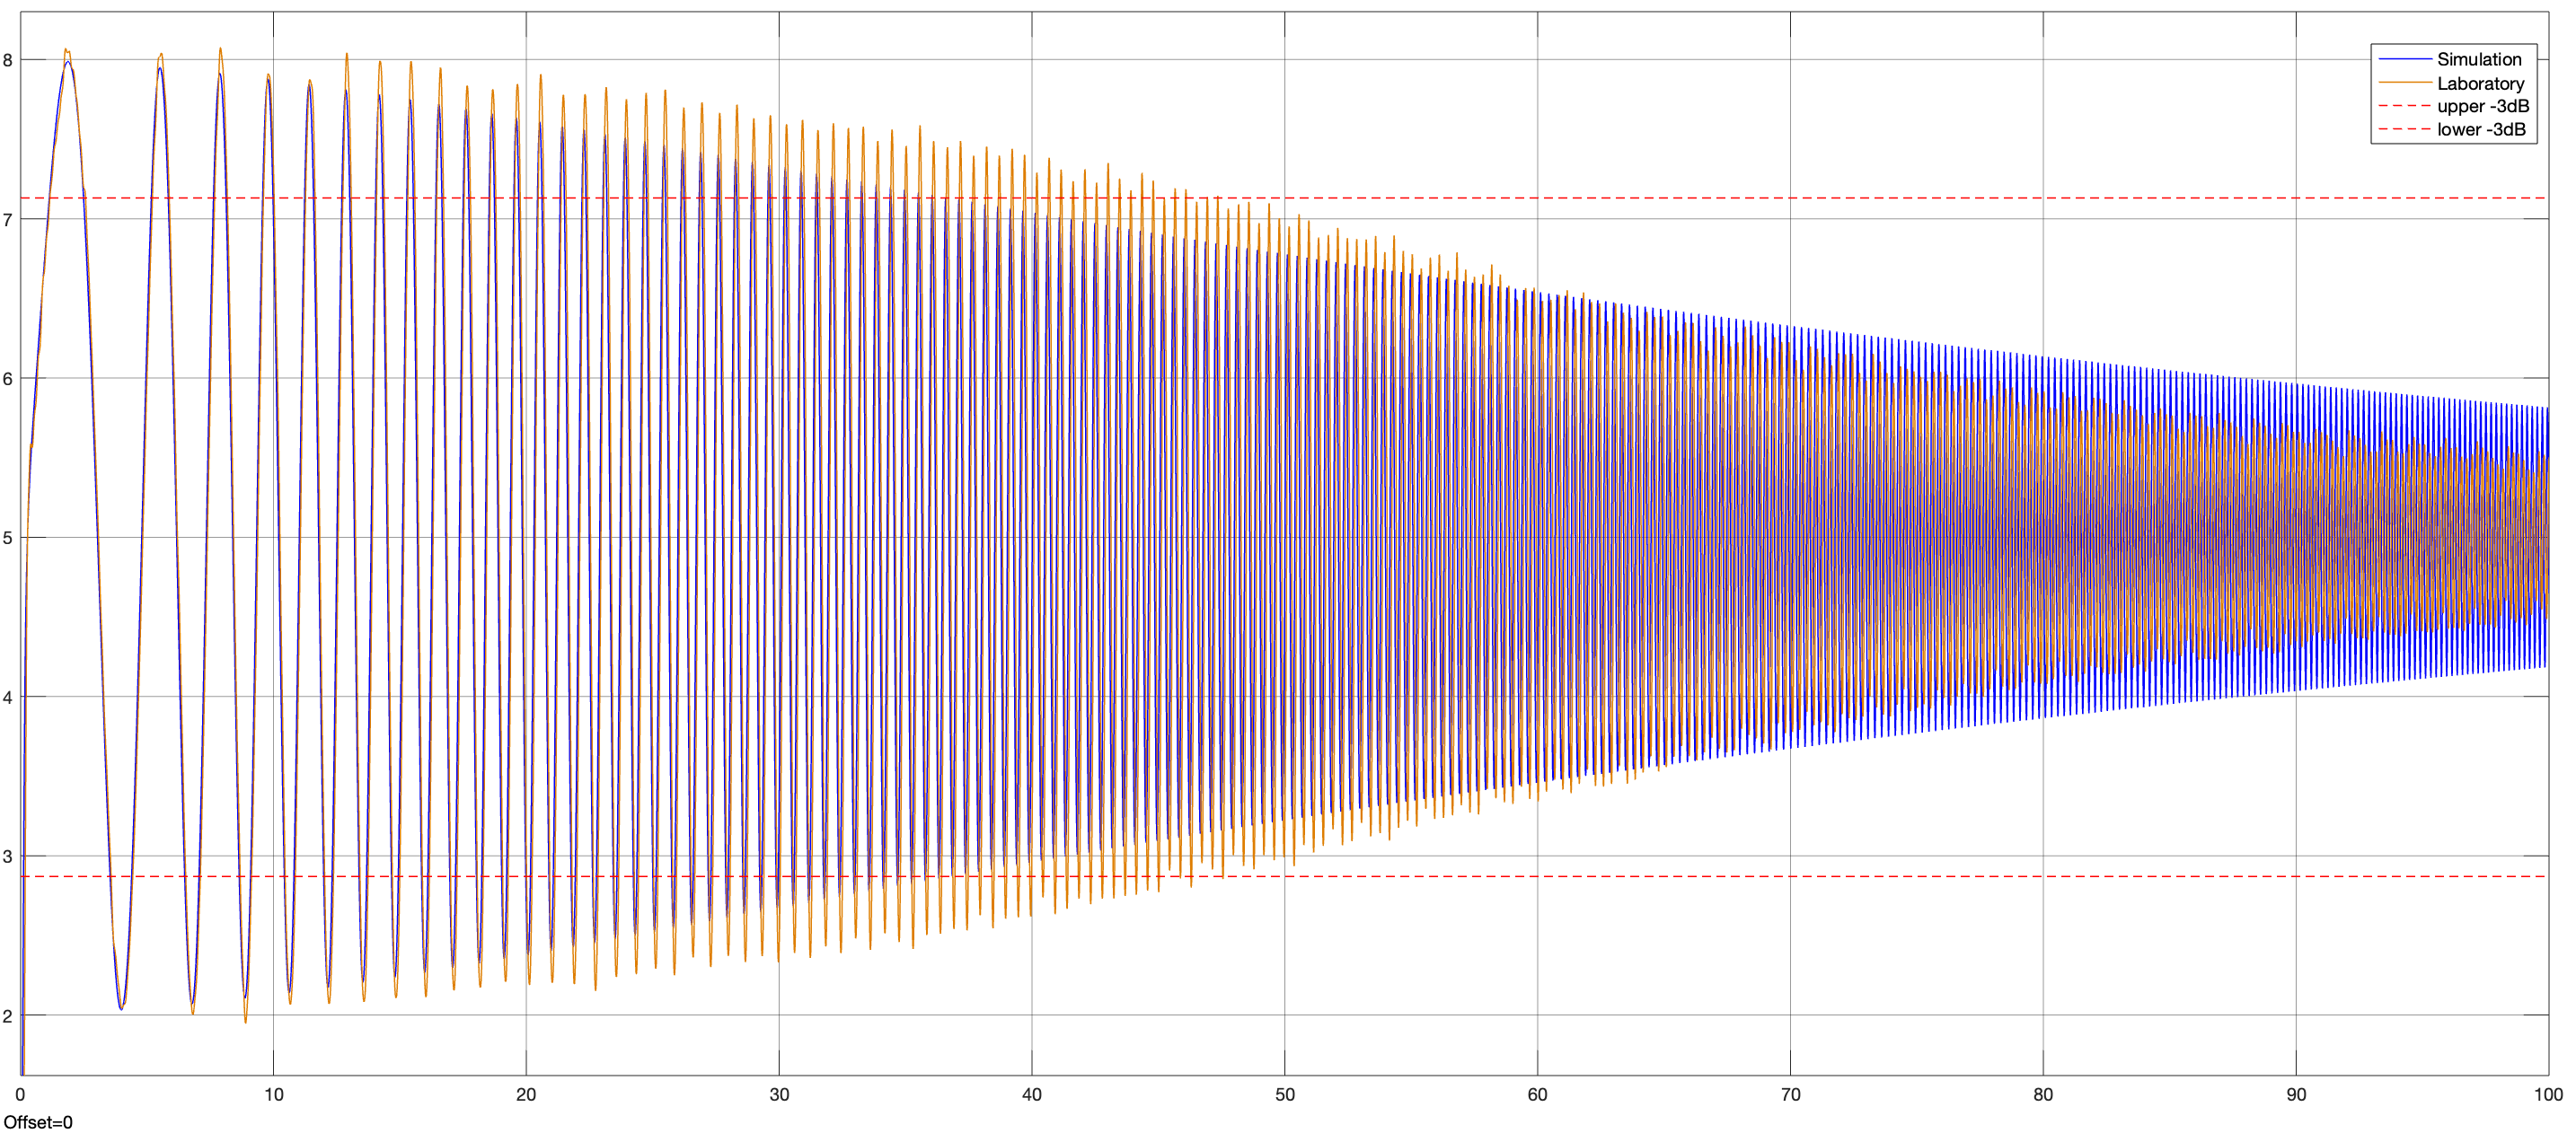
\includegraphics[scale=0.8]{Sine1dof}
	\caption{Sinesweep experiment from 0.1 Hz to 10 Hz in 100s}
\end{figure*}

\begin{figure*}[h]
	\centering
	\begin{subfigure}{0.45\columnwidth}
		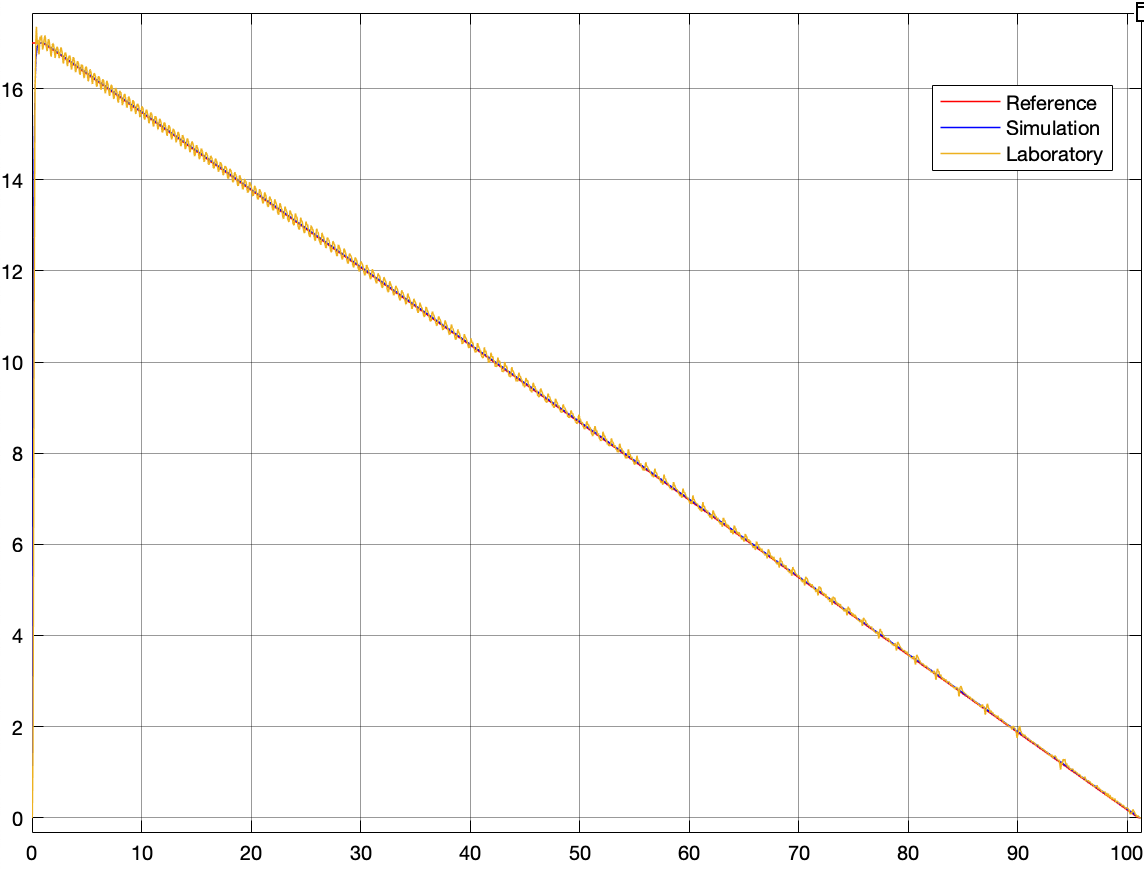
\includegraphics[width=\textwidth]{Ramp1dofa}
		\subcaption{Entire experiment}
	\end{subfigure}
	\begin{subfigure}{0.45\columnwidth}
		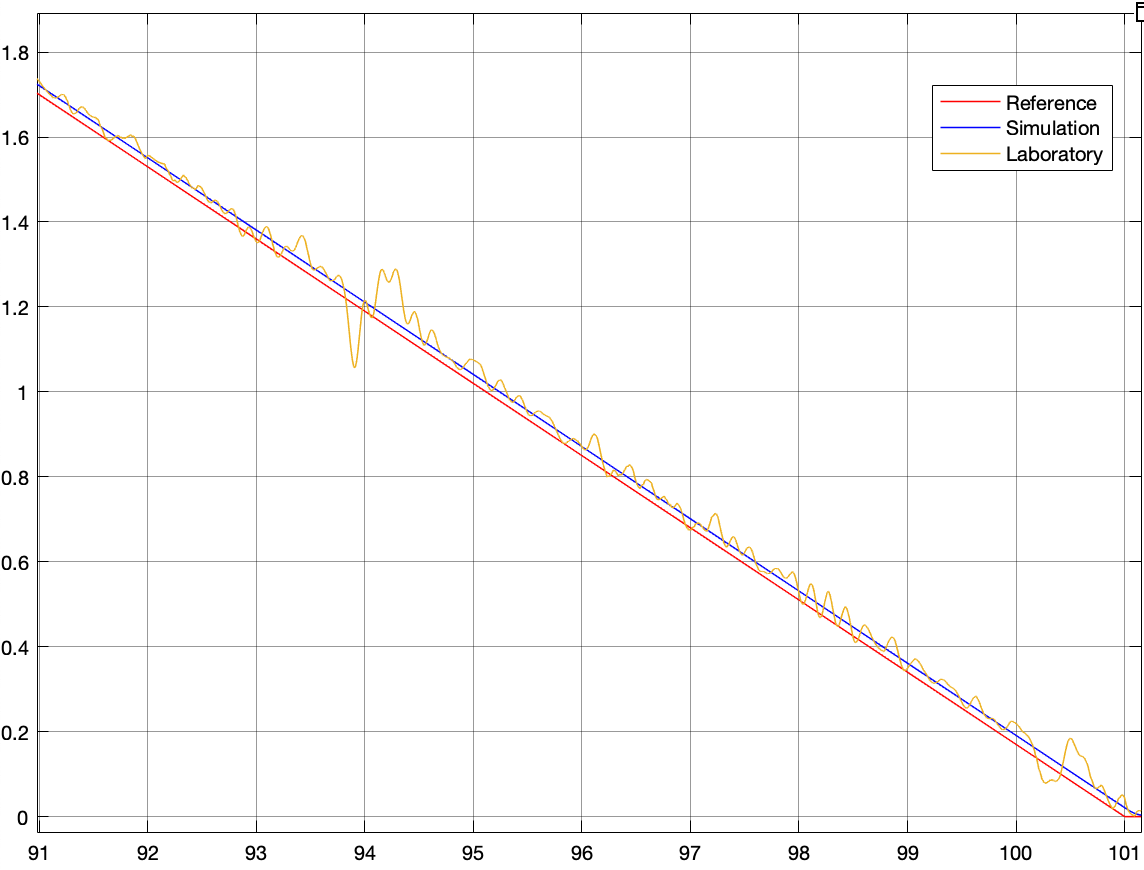
\includegraphics[width=\textwidth]{Ramp1dofb}
		\subcaption{Detail at low speed}
	\end{subfigure}
	\caption{Ramp experiment from 17 rad/s to 0 rad/s in 100s}
	\label{fig:Ramp1dof}
\end{figure*}

\newpage
\subsection{Position Control Loop}
To control the position, we decide to use a cascade strategy: the inner loop controls the speed, whereas the outer one the position. For the first loop we use the same PI structure as explained above, while the position is regulated by using a proportional controller. It is important to remark that the cutting frequency of the position and the speed one must be far enough (about one decade) to assure the frequency decoupling of the two loops. As consequence if we maintain the cutting frequency of the speed loop as decided before ($wc_v$=4.5 rad/s that corresponds to a bandwidth of 8 rad/s), a first possible solution is reached by setting the position cutting frequency equal to 0.8 rad/s. This case is represented in the figure \ref{fig:Bode and Step P 0.8}. From these plots we can see that the overall system is very robust but also very slow.

\begin{figure*}[h]
	\centering
	\begin{subfigure}{0.45\columnwidth}
		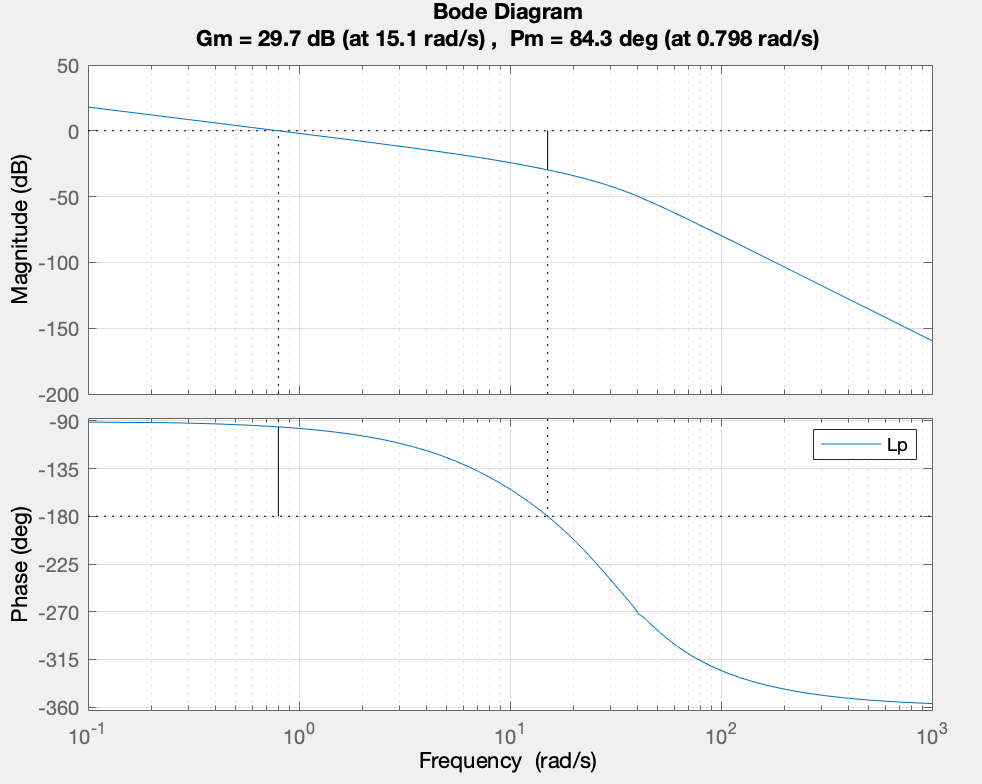
\includegraphics[width=\textwidth]{1_bode0.8}
	\end{subfigure}
	\begin{subfigure}{0.45\columnwidth}
		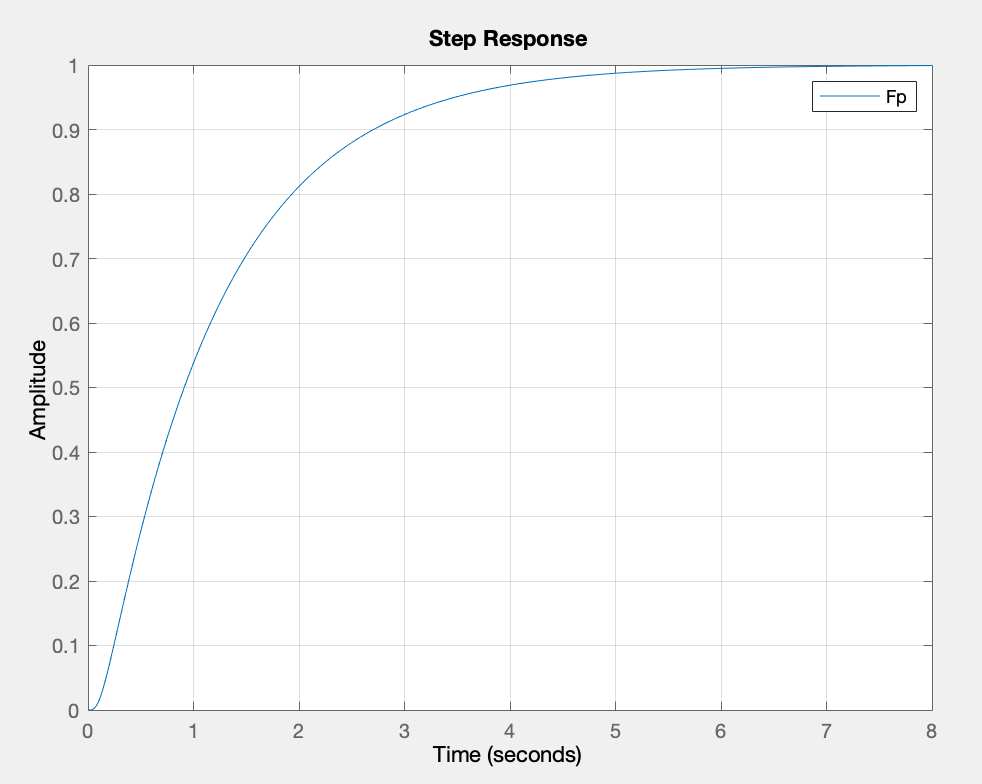
\includegraphics[width=\textwidth]{1_step0.8}
	\end{subfigure}
	\caption{Position control loop with  $wc_{p} $=0.8 rad/s}
	\label{fig:Bode and Step P 0.8}
\end{figure*}

On the other hand, we can accept even a ratio between the speed cutting frequency and the position one up to 50 \%. In this scenario we can fix the proportional gain in order to have a bandwidth around 3 rad/s, and we can notice that the position loop is not so influenced by the inner one.

CONFRONTO TRA SIM E LAB A KPP=3 E WCV=4.5

\newpage
\section{2-DOF System}
We consider as transfer function from voltage to the second mass speed:\\
\\
\[	
G(s)=
\frac{-1.244*10^{8}}{s^5+40.9*s^{4}+4833*s^{3}+1.686*10^{5}*s^{3}+3.327*10^{6}*s+7.355*10^{7}}
\]
\\



\begin{figure*}[h]
	\centering
	\begin{subfigure}{0.4\columnwidth}
		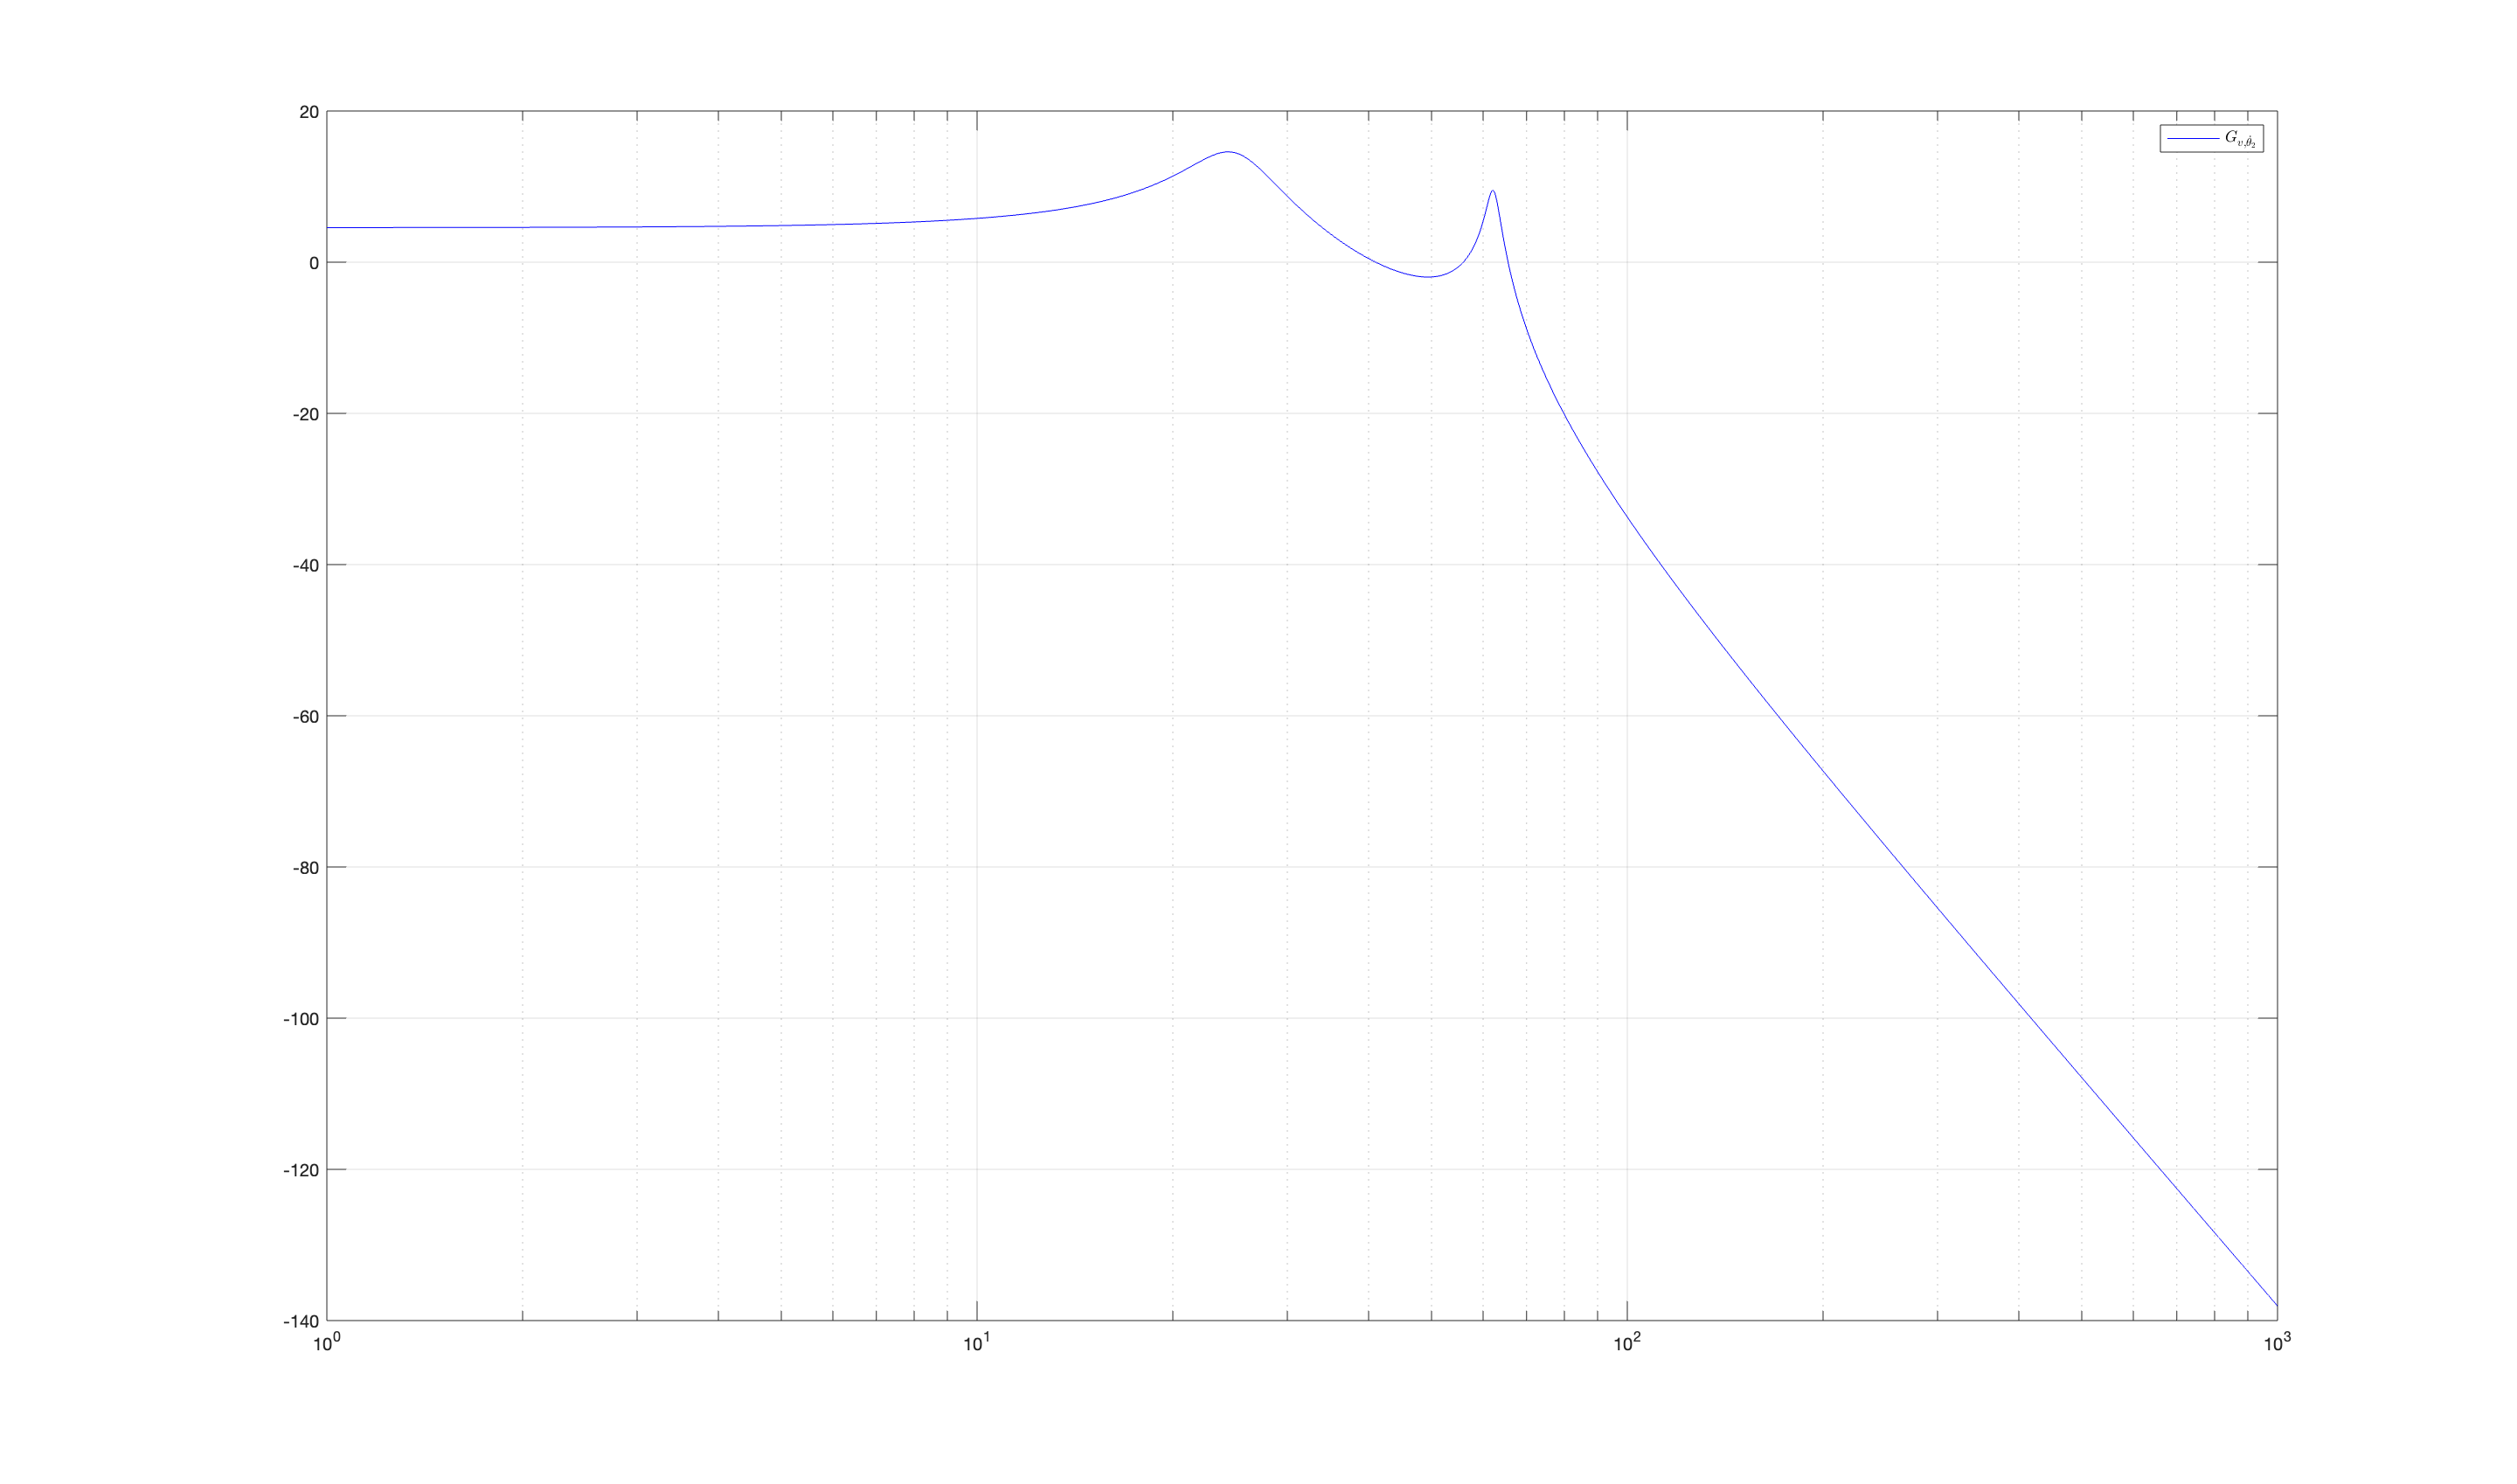
\includegraphics[width=\textwidth]{1_bodeG2}
	\end{subfigure}
	\begin{subfigure}{0.4\columnwidth}
		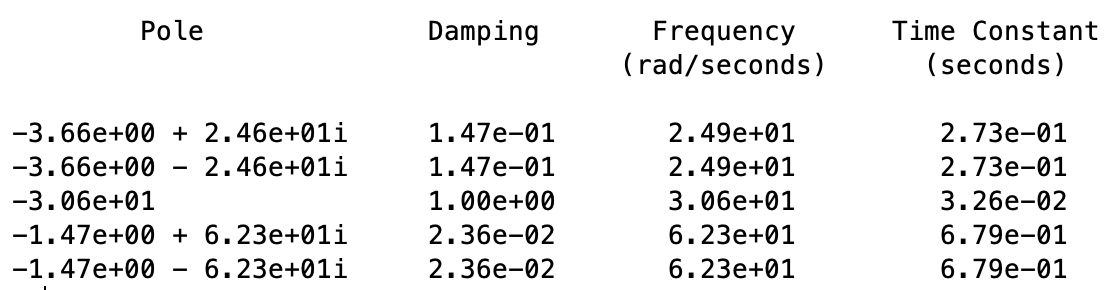
\includegraphics[width=\textwidth]{1_poleG2}
	\end{subfigure}
	\caption{G(s)}
	\label{fig:G(s)2dof}
\end{figure*}

As it is possible to notice in figure \ref{fig:G(s)2dof}, there is a couple of complex conjugated poles with low damping coefficient. We decide so to apply a notch filter, thanks to which we are able to delete these poles and substitute them with a couple of complex conjugated poles at frequency 100 rad/s and a damping coefficient equal to 0.72. The reason why we decide to postpone the poles frequency instead of using the original one is explain in the speed control loop section.


\begin{figure*}[h]
	\centering
	\begin{subfigure}{0.35\columnwidth}
		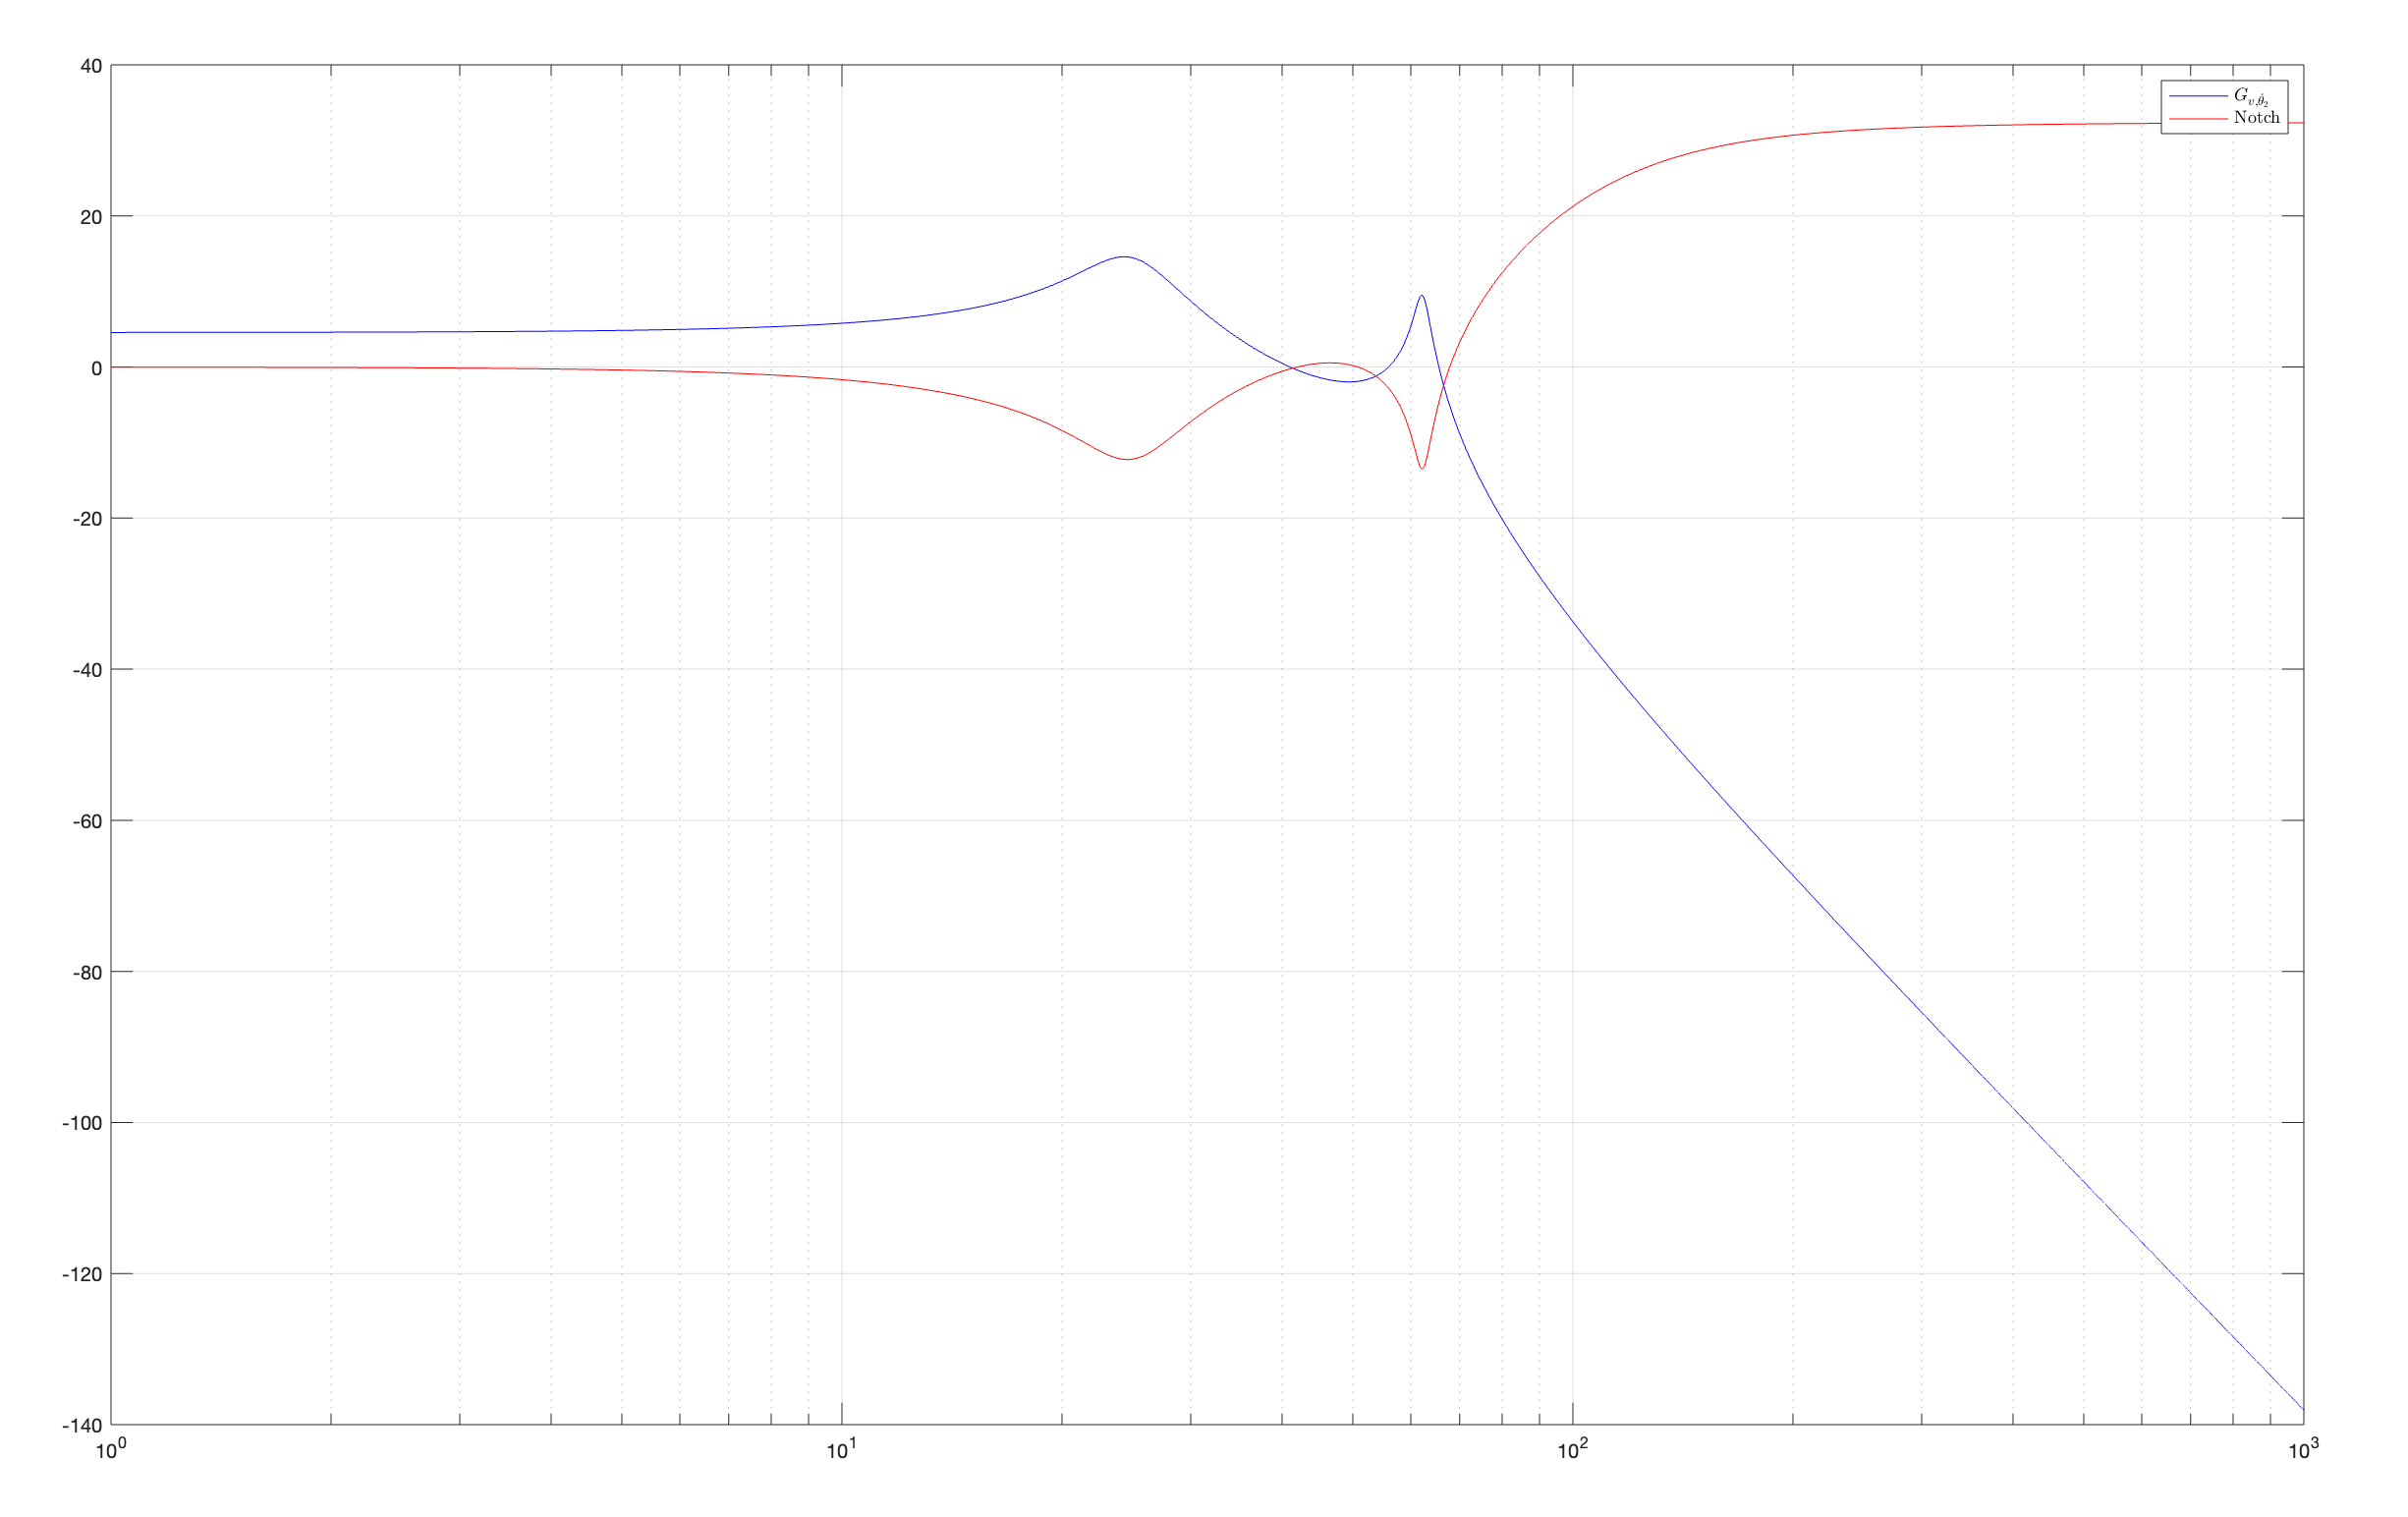
\includegraphics[width=\textwidth]{1Nf_G2}
		\subcaption{Nf(s) and G(s)}
	\end{subfigure}
	\begin{subfigure}{0.35\columnwidth}
		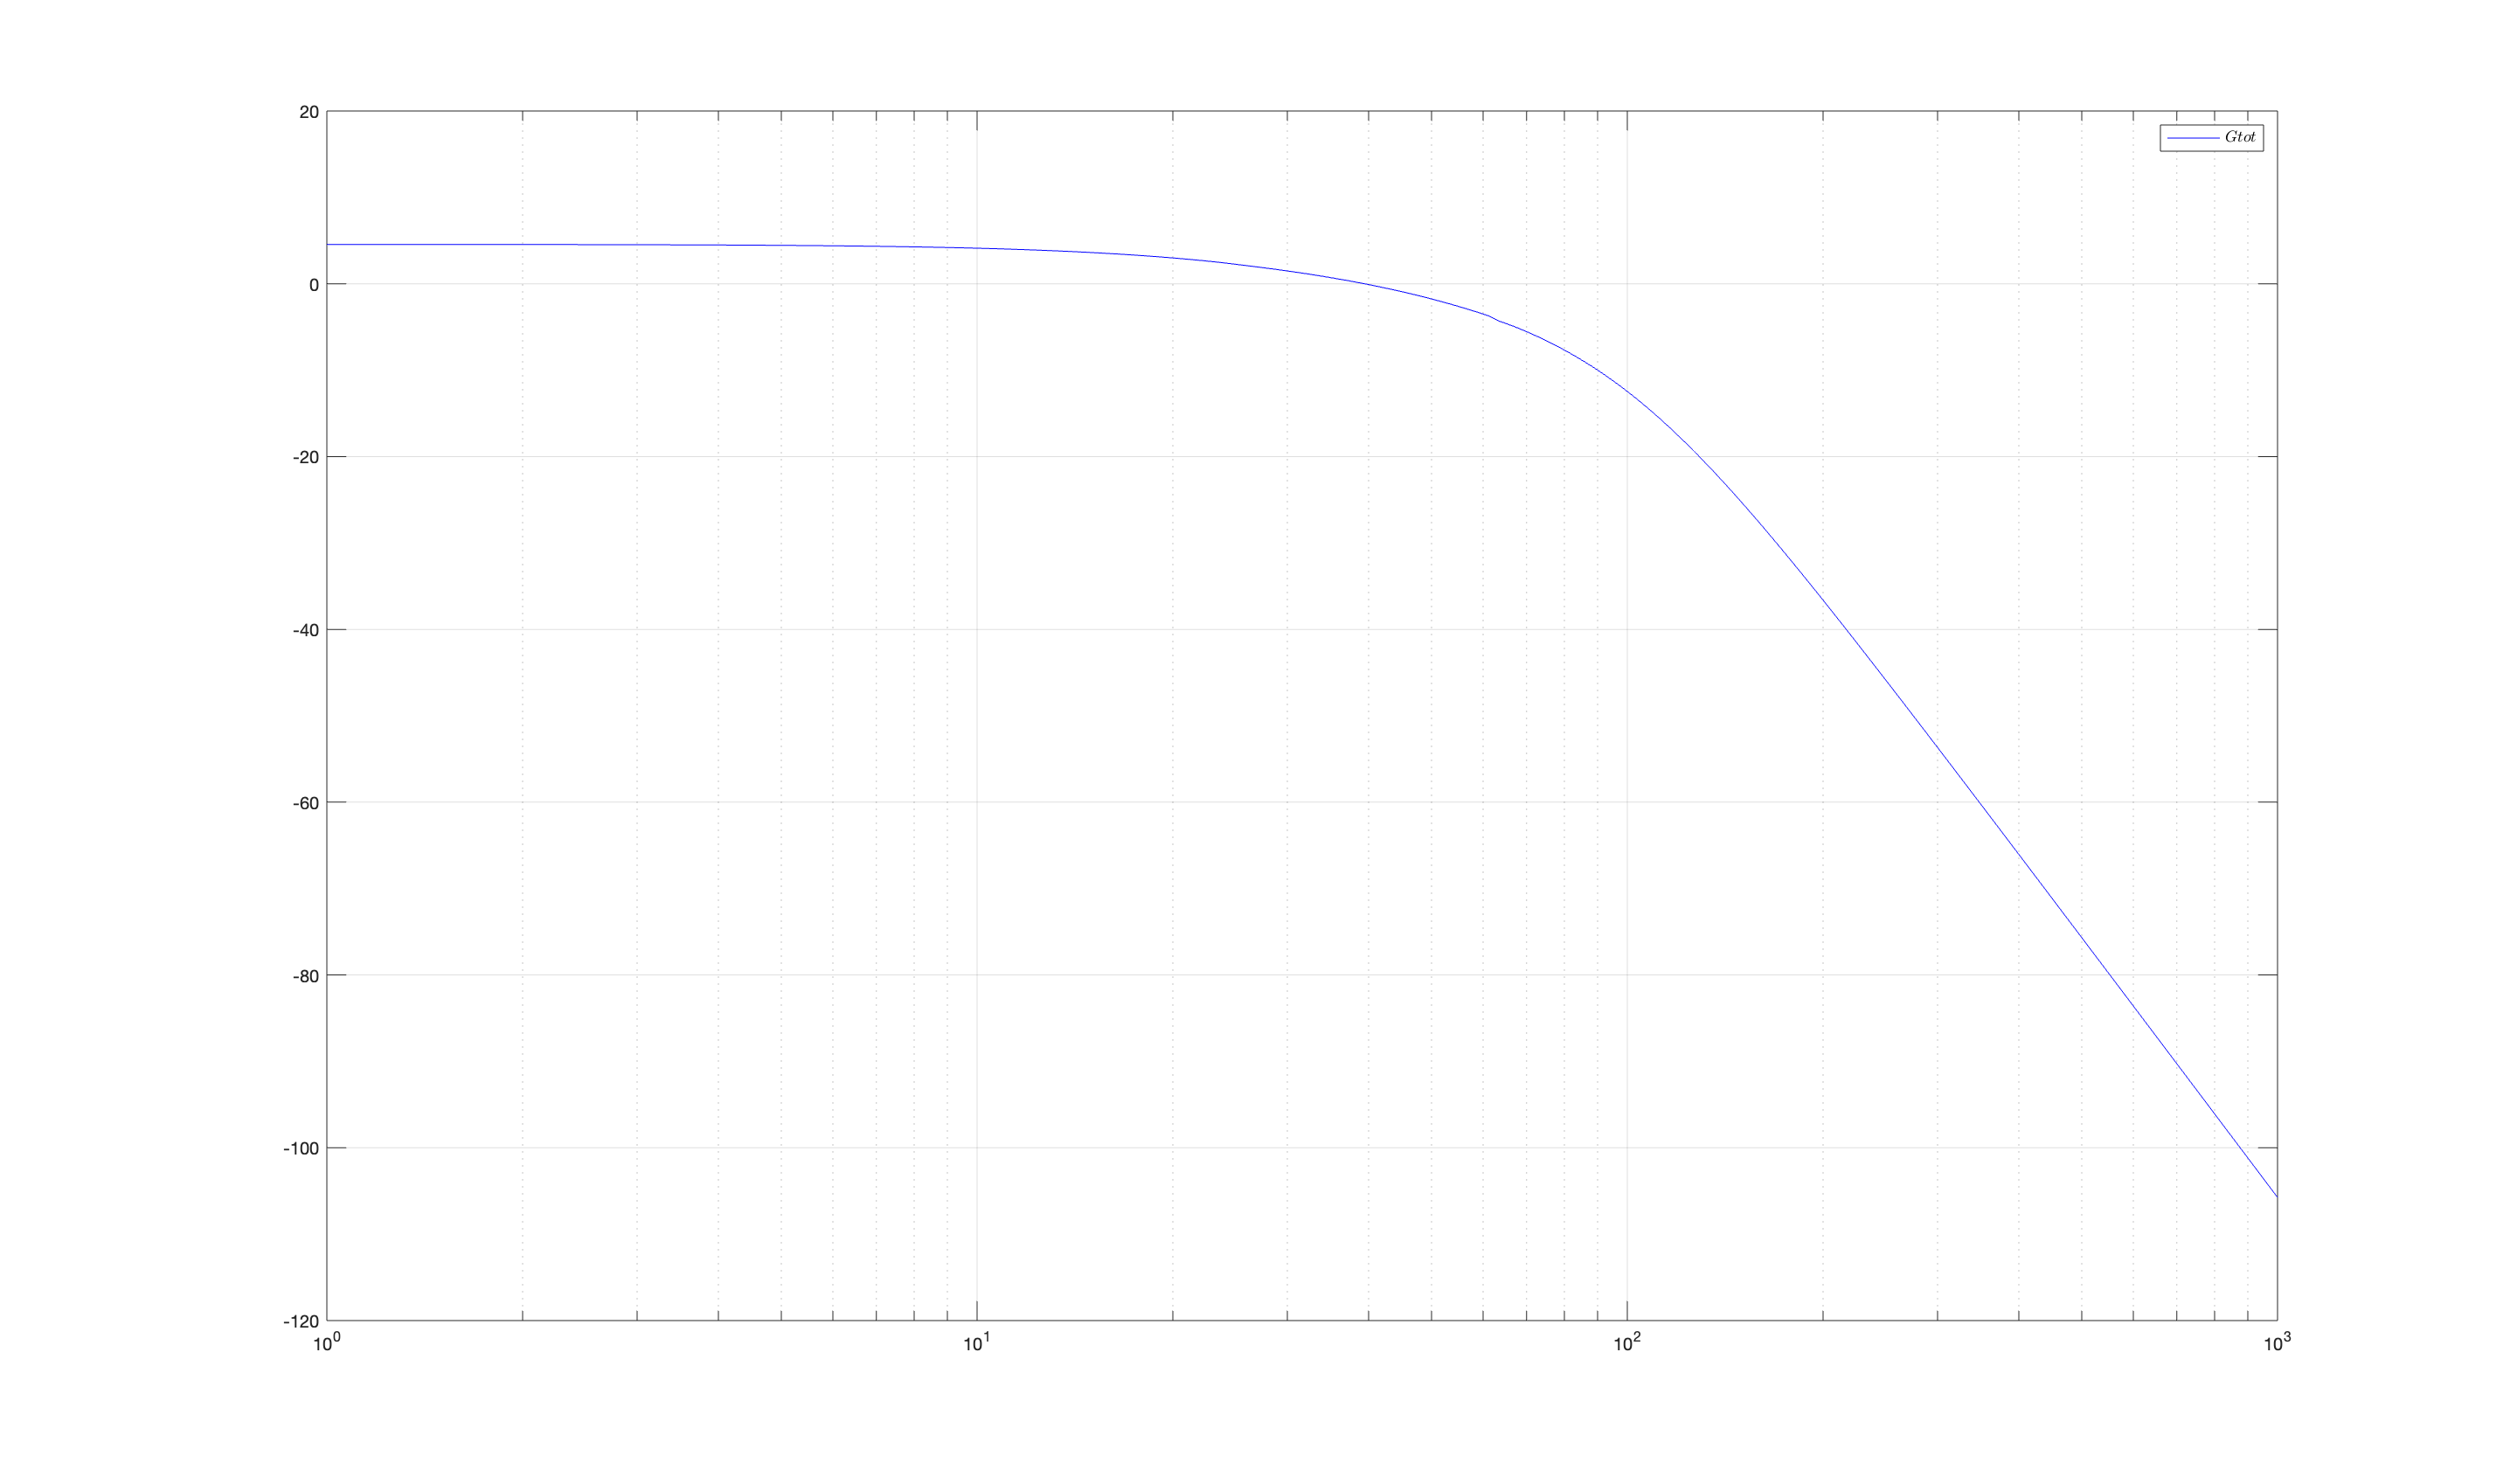
\includegraphics[width=\textwidth]{1_G2tot}
		\subcaption{$G_{tot}$(s)}
	\end{subfigure}
	\caption{Plant G(s) with Notch Filter Nf(s): $G_{tot}$(s)}
	\label{fig:Plant G(s)with Notch Filter2}
\end{figure*}


Applying the notch filter represented in figure \ref{fig:Plant G(s)with Notch Filter2}(a), we obtain the plant $G_{tot}$(s) of figure \ref{fig:Plant G(s)with Notch Filter2}(b) that is the one we are going to control.

\newpage 
\subsection{Speed Control Loop}
We use a PI-regulator enriched with an anti-wind-up structure; we decided then to cancel out the real pole at 30.6 rad/s.
\\
\[
R(s)=-wc_v
\frac{\frac{s}{30.6}+1}{s}
\]
\\
As in the 1-DOF scenario, the presence of the Notch Filter postpones the cutting frequency imposed by the PI, indeed the wcv written in the legends below, are referred to the same parameter written in R and not to the real bandwidth of the speed-loop.







